\documentclass[aspectratio=169]{beamer}
\usepackage{amsmath, amssymb, amsfonts, amsthm}
\usepackage{cancel}
\usepackage[output-complex-root=j]{siunitx}
\usepackage[american, nooldvoltagedirection]{circuitikz}
\usepackage{bm}
\usepackage{listings}
\usepackage{graphicx}
\usepackage{hyperref}

\usetheme{Berkeley}
\usefonttheme[onlymath]{serif}
\AtBeginSection[]{
    \begin{frame}
    \vfill
    \centering
    \begin{beamercolorbox}[sep=8pt,center,shadow=false,rounded=false]{title}
    \usebeamerfont{title}\insertsectionhead\par
    \end{beamercolorbox}
    \vfill
    \end{frame}
}

\newcommand{\N}{\mathbb{N}}
\newcommand{\Z}{\mathbb{Z}}
\newcommand{\Q}{\mathbb{Q}}
\newcommand{\R}{\mathbb{R}}
\newcommand{\C}{\mathbb{C}}

\title{EECS 16B CSM}
\author{Bryan Ngo}
\date{2022-03-01}
\institute{UC Berkeley}

\begin{document}

\begin{frame}
    \maketitle
\end{frame}

\maketitle

\section{Phasors}

\begin{frame}{Phasors}
    \begin{itemize}
        \item Encodes information about any sinusoid: voltage, current, etc.
        \item If frequency is constant, then uniquely identifies
    \end{itemize}
    \begin{align}
        % A \cos(\omega t + \phi) = \Re\{A e^{j (\omega t + \phi)}\} = \Re\{\underbrace{A e^{j \phi}}_{\text{phasor}} e^{j \omega t}\}
        x(t) = A \cos(\omega t + \phi) &= \frac{A}{2} \left(e^{j (\omega t + \phi)} + e^{-j (\omega t + \phi)}\right) \\
        &= \frac{A}{2} \left(e^{j \omega t} e^{j \phi} + \overline{e^{j \omega t} e^{j \phi}}\right) \\
        \iff \widetilde{X} &= \frac{A}{2} e^{j \phi}
    \end{align}
\end{frame}

\begin{frame}{Properties}
    Given \(x_1(t) = \widetilde{X}_1 e^{j \omega t} + \overline{\widetilde{X}_1 e^{j \omega t}}, x_2(t) = \widetilde{X}_2 e^{j \omega t} + \overline{\widetilde{X}_2 e^{j \omega t}}\) with phasors \(\widetilde{X}_{1, 2}\),
    \begin{itemize}
        \item Uniqueness: \(x_1(t) = x_2(t) \implies \widetilde{X}_1 = \widetilde{X}_2\)
        \item Linearity: \(a_1 x_1(t) + a_2 x_2(t) \implies a_1 \widetilde{X}_1 + a_2 \widetilde{X}_2\) for \(a_{1, 2} \in \mathbb{R}\)
        \item Differentiation: \(x(t) \iff \widetilde{X} \implies \frac{d}{dt} x(t) = \frac{d}{dt} \left(\widetilde{X} e^{j \omega t} + \overline{\widetilde{X} e^{j \omega t}}\right) = j \omega \left(\widetilde{X} e^{j \omega t} + \overline{\widetilde{X} e^{j \omega t}}\right) \iff j \omega \widetilde{X}\)
    \end{itemize}
\end{frame}

\begin{frame}{Circuits \& Phasors}{KVL}
    \begin{center}
        \begin{circuitikz}\draw
            (0, 0) to[generic, v^=~] (0, 2) to[generic, v^=~] (2, 2) to[generic, v^=~] (2, 0) to[generic, v^=~] (0, 0);
            \draw[thin, <-, ] (1,1) ++(-60:0.5) arc (-60:170:0.5);
        \end{circuitikz}
    \end{center}
    \begin{equation}
        \sum_i \widetilde{V}_i = 0
    \end{equation}
\end{frame}

\begin{frame}{Circuits \& Phasors (cont.)}{KCL}
    \begin{center}
        \begin{circuitikz}\draw
            (-2, 2) to[generic, i=~] (0, 2) to[generic, i>^=~] (2, 2)
            (0, 0) to[generic, i=~] (0, 2)
        ;\end{circuitikz}
    \end{center}
    \begin{equation}
        \sum \widetilde{I}_{out} = \sum \widetilde{I}_{in}
    \end{equation}
\end{frame}

\begin{frame}{Circuits \& Phasors (cont.)}{Ohm's Law}
    \begin{center}
        \begin{circuitikz}\draw
            (0, 0) to[generic=\(Z\), v=\(V\), i>^=\(I\)] (4, 0)
        ;\end{circuitikz}
    \end{center}
    \begin{equation}
        \widetilde{V} = \widetilde{I} \underbrace{Z}_{\text{impedance}}
    \end{equation}
\end{frame}

\begin{frame}{Passive Elements \& Phasors}
    \scalebox{0.75}{
        \begin{circuitikz}\draw
            (0, 2) to[R=\(R\), v=\(V\), i>^=\(I\)] (0, 0)
        ;\end{circuitikz}
    }
    \begin{equation}
        \widetilde{V} = \widetilde{I} R
    \end{equation}
    \scalebox{0.75}{
        \begin{circuitikz}[scale=0.8]\draw
            (0, 2) to[L=\(L\), v=\(V\), i>^=\(I\)] (0, 0)
        ;\end{circuitikz}
    }
    \begin{equation}
        \widetilde{V} = L \frac{d}{dt} \widetilde{I} = j \omega L \widetilde{I}
    \end{equation}
    \scalebox{0.75}{
        \begin{circuitikz}[scale=0.8]\draw
            (0, 2) to[C=\(C\), v=\(V\), i>^=\(I\)] (0, 0)
        ;\end{circuitikz}
    }
    \begin{equation}
        \widetilde{I} = C \frac{d}{dt} \widetilde{V} = j \omega C \widetilde{V} \implies \widetilde{V} = \frac{1}{j \omega C} \widetilde{I}
    \end{equation}
\end{frame}

\section{Filters}

\begin{frame}
    \frametitle{Why?}

    \begin{itemize}
        \item allows us to isolate desired frequency ranges
        \item color organ: basically just a spectrogram
        \item \href{https://youtu.be/OBM5T5_kgdI}{Afrotechmods video}
    \end{itemize}
\end{frame}

\begin{frame}
    \frametitle{Types}

    \begin{itemize}
        \item low-pass: let in low \(\omega\)
        \item high-pass: let in high \(\omega\)
        \item band-pass: let in range of \(\omega\)
        \item band-stop: block out range of \(\omega\)
    \end{itemize}

\end{frame}

\begin{frame}
    \frametitle{Transfer Functions}
    
    \begin{align}
        H(j \omega) = \frac{V_{out}}{V_{in}} &= \frac{(j \omega)^{N_z}}{(j \omega)^{N_p}} \frac{\alpha_0 + (j \omega) \alpha_1 + \cdots + (j \omega)^n \alpha_n}{\beta_0 + (j \omega) \beta_1 + \cdots + (j \omega)^m \beta_m} \\
        &= K \frac{(j \omega)^{N_z}}{(j \omega)^{N_p}} \frac{\left(1 + j \frac{\omega}{\omega_{z1}}\right) \left(1 + j \frac{\omega}{\omega_{z2}}\right) \cdots \left(1 + j \frac{\omega}{\omega_{zn}}\right)}{\left(1 + j \frac{\omega}{\omega_{p1}}\right) \left(1 + j \frac{\omega}{\omega_{p2}}\right) \cdots \left(1 + j \frac{\omega}{\omega_{pn}}\right)}
    \end{align}
    \begin{itemize}
        \item \(N_z\): number of zeroes
        \item \(N_p\): number of poles
        \item \(\omega_{zn}\): \(n\)-th zero
        \item \(\omega_{pn}\): \(n\)-th pole
    \end{itemize}
\end{frame}

\section{Bode Plots}

\begin{frame}
    \frametitle{Definition}
    \begin{columns}
        \column[]{0.5\textwidth}
        \centering
        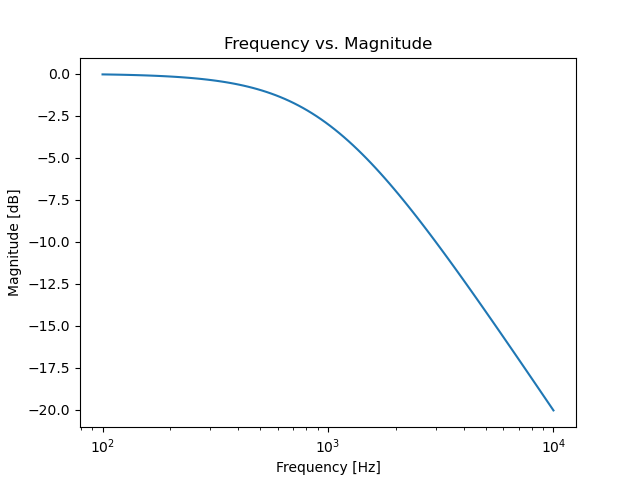
\includegraphics[width=0.8\textwidth]{Figure_1.png}

        \column[]{0.5\textwidth}
        \centering
        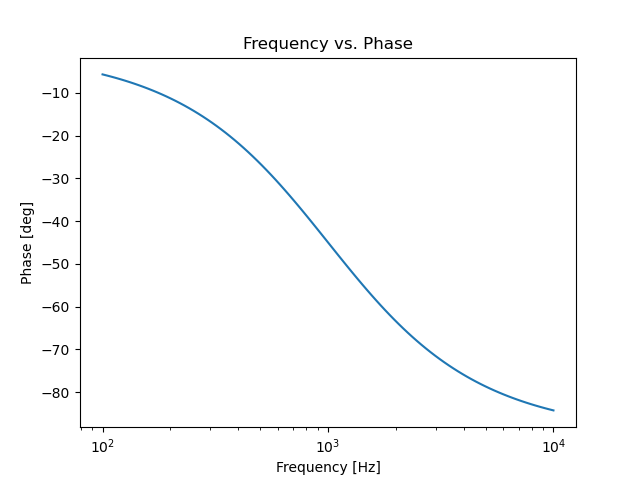
\includegraphics[width=0.8\textwidth]{Figure_2.png}
    \end{columns}
    \begin{itemize}
        \item comes in pairs: magnitude \& phase
        \item above: low-pass filter
    \end{itemize}
\end{frame}

\begin{frame}
    \frametitle{Features}

    \begin{itemize}
        \item magnitude
        \begin{itemize}
            \item \(x\)-axis: log frequency (\si{\hertz})
            \item \(y\)-axis: \(|H(j \omega)|\) (\si{\deci\bel} or intensity)
            \item \textbf{cutoff frequency}: \(|H(j \omega)| = \frac{1}{\sqrt{2}} = \SI{-3}{\deci\bel}\)
        \end{itemize}
        \item phase
        \begin{itemize}
            \item \(x\)-axis: log frequency (\si{\hertz})
            \item \(y\)-axis: phase offset (\si{\degree} or \si{\radian})
        \end{itemize}
    \end{itemize}
\end{frame}

\begin{frame}
    \frametitle{Why?}

    \begin{itemize}
        \item allows us to characterize a filter very fast
        \item quick visual tool
    \end{itemize}
\end{frame}

\begin{frame}
    \frametitle{Resonance}

    \begin{itemize}
        \item whenever you see an inductor \& a capacitor
        \item energy is oscillating back and forth
        \item when voltage is at resonant frequency \(\frac{1}{\sqrt{LC}}\), inductor and capacitor act as short
    \end{itemize}
\end{frame}

\end{document}
